\documentclass[journal,12pt,twocolumn]{IEEEtran}
\usepackage{amsthm}
\usepackage{gensymb}
\usepackage{setspace}
\singlespacing
\usepackage[cmex10]{amsmath}
\usepackage{bm}

\usepackage{cases}
\usepackage{mathrsfs}
\usepackage{cite}
\usepackage{stfloats}
\usepackage{mathtools}
\usepackage[breaklinks=true]{hyperref}
\usepackage{graphicx}
\usepackage{subfig}
\usepackage{txfonts}
\usepackage{longtable}
\usepackage{multirow}
\usepackage{tfrupee}
\usepackage{enumitem}
\usepackage{tikz}
\usepackage{steinmetz}
\usepackage{verbatim}
\usepackage{circuitikz}
\usepackage{tkz-euclide}





\usetikzlibrary{calc,math}
\usepackage{listings}
    \usepackage{color}                                            %%
    \usepackage{array}                                            %%
    \usepackage{longtable}                                        %%
    \usepackage{calc}                                             %%
    \usepackage{multirow}                                         %%
    \usepackage{hhline}                                           %%
    \usepackage{ifthen}                                           %%
    \usepackage{lscape}     
\usepackage{multicol}
\usepackage{chngcntr}

\DeclareMathOperator*{\Res}{Res}

\renewcommand\thesection{\arabic{section}}
\renewcommand\thesubsection{\thesection.\arabic{subsection}}
\renewcommand\thesubsubsection{\thesubsection.\arabic{subsubsection}}

\renewcommand \thesectiondis{\arabic{section}}
\renewcommand\thesubsectiondis{\thesectiondis.\arabic{subsection}}
\renewcommand\thesubsubsectiondis{\thesubsectiondis.\arabic{subsubsection}}


\hyphenation{op-tical net-works semi-conduc-tor}
\def\inputGnumericTable{}                                 %%

\lstset{
%language=C,
frame=single, 
breaklines=true,
columns=fullflexible
}
\begin{document}

\newcommand{\BEQA}{\begin{eqnarray}}
\newcommand{\EEQA}{\end{eqnarray}}
\newcommand{\define}{\stackrel{\triangle}{=}}
\bibliographystyle{IEEEtran}
\raggedbottom
\setlength{\parindent}{0pt}
\providecommand{\mbf}{\mathbf}
\providecommand{\pr}[1]{\ensuremath{\Pr\left(#1\right)}}
\providecommand{\qfunc}[1]{\ensuremath{Q\left(#1\right)}}
\providecommand{\sbrak}[1]{\ensuremath{{}\left[#1\right]}}
\providecommand{\lsbrak}[1]{\ensuremath{{}\left[#1\right.}}
\providecommand{\rsbrak}[1]{\ensuremath{{}\left.#1\right]}}
\providecommand{\brak}[1]{\ensuremath{\left(#1\right)}}
\providecommand{\lbrak}[1]{\ensuremath{\left(#1\right.}}
\providecommand{\rbrak}[1]{\ensuremath{\left.#1\right)}}
\providecommand{\cbrak}[1]{\ensuremath{\left\{#1\right\}}}
\providecommand{\lcbrak}[1]{\ensuremath{\left\{#1\right.}}
\providecommand{\rcbrak}[1]{\ensuremath{\left.#1\right\}}}
\theoremstyle{remark}
\newtheorem{rem}{Remark}
\newcommand{\sgn}{\mathop{\mathrm{sgn}}}
\providecommand{\abs}[1]{\vert#1\vert}
\providecommand{\res}[1]{\Res\displaylimits_{#1}} 
\providecommand{\norm}[1]{\lVert#1\rVert}
%\providecommand{\norm}[1]{\lVert#1\rVert}
\providecommand{\mtx}[1]{\mathbf{#1}}
\providecommand{\mean}[1]{E[ #1 ]}
\providecommand{\fourier}{\overset{\mathcal{F}}{ \rightleftharpoons}}
%\providecommand{\hilbert}{\overset{\mathcal{H}}{ \rightleftharpoons}}
\providecommand{\system}{\overset{\mathcal{H}}{ \longleftrightarrow}}
	%\newcommand{\solution}[2]{\textbf{Solution:}{#1}}
\newcommand{\solution}{\noindent \textbf{Solution: }}
\newcommand{\cosec}{\,\text{cosec}\,}
\providecommand{\dec}[2]{\ensuremath{\overset{#1}{\underset{#2}{\gtrless}}}}
\newcommand{\myvec}[1]{\ensuremath{\begin{pmatrix}#1\end{pmatrix}}}
\newcommand{\mydet}[1]{\ensuremath{\begin{vmatrix}#1\end{vmatrix}}}
\numberwithin{equation}{subsection}
\makeatletter
\@addtoreset{figure}{problem}
\makeatother
\let\StandardTheFigure\thefigure
\let\vec\mathbf
\renewcommand{\thefigure}{\theproblem}
\def\putbox#1#2#3{\makebox[0in][l]{\makebox[#1][l]{}\raisebox{\baselineskip}[0in][0in]{\raisebox{#2}[0in][0in]{#3}}}}
     \def\rightbox#1{\makebox[0in][r]{#1}}
     \def\centbox#1{\makebox[0in]{#1}}
     \def\topbox#1{\raisebox{-\baselineskip}[0in][0in]{#1}}
     \def\midbox#1{\raisebox{-0.5\baselineskip}[0in][0in]{#1}}
\vspace{3cm}
\title{Assignment8}%number
\author{CS20Btech11035 -NYALAPOGULA MANASWINI}
\maketitle
\newpage
\bigskip

\renewcommand{\thefigure}{\theenumi}
\renewcommand{\thetable}{\theenumi}
Download python code from 
\begin{lstlisting}
https://github.com/N-Manaswini23/Assignment8/tree/main/python%20codes
\end{lstlisting}
%
Download latex code from 
\begin{lstlisting}
https://github.com/N-Manaswini23/Assignment8/blob/main/assignment8.tex
\end{lstlisting}
%

\section*{CSIR UGC JUNE 2013 QUESTION 70}
Let $X$ and $Y$ be independent random variables each following a uniform distribution on $(0,1)$.Let $W=XI_{\{Y\leq X^2\}}$,where $I_A$ denotes the indicator function of set $A$.Then which of the following statements are true? \\
\begin{enumerate}
\item The cumulative distribution function of $W$ is given by
\begin{align}
  F_W(t)=t^2I_{\{0\leq t \leq 1\}}+ I_{\{t > 1\}}
\end{align}
\item $P\sbrak{W>0}=\frac{1}{3}$
\item The cumulative distribution function of $W$ is continuous
\item The cumulative distribution function of $W$ is given by
\begin{align}
  F_W(t)=\brak{\frac{2+t^3}{3}}I_{\{0\leq t \leq 1\}}+ I_{\{t > 1\}}
\end{align}
\end{enumerate}

\section*{ANSWER}
Options $2$ and $4$ are correct.

\section*{SOLUTION}

Given $X$ and $Y$ be two independent random\\
variables. \\
Given $W=XI_{\{Y\leq X^2\}}$ \\
$X \in \brak{0,1}$ , $Y \in \brak{0,1}$ , $W \in [0,1)$\\
\begin{enumerate}
\item The PDF for $X$ is
\begin{align}
p_X(x) = 
\begin{cases}
     1 & 0 < x  < 1 \\
     0 & otherwise 
\end{cases}\label{1}
\end{align}
\item The CDF for $X$ is
\begin{align}
F_{X}(x)  = 
\begin{cases}
      0 & x \leq 0 \\
      x & 0 < x < 1 \\
      1 & otherwise
\end{cases}  \label{eq:2}
\end{align}
\item The PDF for $Y$ is
\begin{align}
p_{Y}(y)  = 
\begin{cases}
      1 & 0 < y < 1 \\
      0 & otherwise 
\end{cases} \label{3}
\end{align}
\item The CDF for $Y$ is
\begin{align}
F_{Y}(y)  = 
\begin{cases}
      0 & y \leq 0 \\
      y & 0 < y < 1 \\
      1 & otherwise 
\end{cases}\label{4}
\end{align}
\item $I_{\{Y\leq X^2\}}$ is defined as follows
\begin{align} 
I_{\{Y\leq X^2\}} =
\begin{cases}
    1 & y \leq x^2  \\
    0 & otherwise 
\end{cases} \label{5}
\end{align}
\item $W$ is defined as follows
\begin{align}
W  = 
\begin{cases}
    x & y \leq x^2 \\
    0 & otherwise
\end{cases}  \label{6}
\end{align}
From \eqref{6}
\begin{align}
p_W(W=0) &= \Pr(I_{\{Y\leq X^2\}}=0) \\
         &=\Pr(x^2 <y) \label{7}
\end{align}
\item Let $Z=X^2-Y$ be a random variable where $Z \in \brak{-1,1}$
\begin{align}
F_{X^2}(u)&=\Pr(X^2 \leq u) \\
          &=\Pr(X \leq \sqrt{u}) \\
          &=F_X(\sqrt{u}) \label{8}
\end{align}
\item From \eqref{eq:2},The CDF for $X^2$ is
\begin{align}
F_{X^2}(u)  = 
\begin{cases}
      0 & u \leq 0 \\
      \sqrt{u} & 0 < u < 1 \\
      1 & otherwise
\end{cases} \label{9}
\end{align}
\item The PDF for $X^2$ is
\begin{align}
p_{X^2}(u)  = 
\begin{cases}
      \frac{1}{2\sqrt{u}} & 0 < u < 1 \\
      0 & otherwise
\end{cases} \label{10}
\end{align}
\begin{align}
F_{\{-Y\}}(v)&=\Pr(-Y \leq v) \\
          &=\Pr(Y \geq -v) \\
          &=1-F_Y(-v) \label{11}
\end{align}
\item From \eqref{4},The CDF for $(-Y)$ is
\begin{align}
F_{\{-Y\}}(v)  = 
\begin{cases}
      0 & v \leq -1\\
      1+v & -1 < v < 0 \\
      1 & otherwise 
\end{cases}\label{12}
\end{align}
\item The PDF for $(-Y)$ is
\begin{align}
p_{\{-Y\}}(v)  = 
\begin{cases}
      1 & -1 < v < 0 \\
      0 & otherwise
\end{cases} \label{p-y}
\end{align}
\item $Z=X^2-Y$ $\implies  z=u+v$\\
Using convolution
\begin{align}
p_Z(z)=\int_{- \infty}^{\infty} p_{X^2}(z-v)p_{\{-Y\}}(v) \mathrm{dv} \label{pz}
\end{align}
Solving \eqref{pz} using \eqref{p-y},\eqref{10} for $z \in (-1,1)$, we get PDF of $Z$ as follows
\begin{align}
p_{Z}(z)  = 
\begin{cases}
      \sqrt{z+1} & -1 < z \leq 0 \\
      1-\sqrt{z} & 0 < z <1 \\
      0 & otherwise 
\end{cases} \label{13}
\end{align}
\item CDF of $Z$ as follows
\begin{align}
F_{Z}(z)  = 
\begin{cases}
      \frac{2}{3}{(z+1)}^\frac{3}{2} & -1 < z \leq 0 \\
      z-\frac{2}{3}{z}^\frac{3}{2} & 0 < z < 1 \\
      1 & otherwise
\end{cases} \label{14}
\end{align}
\item using \eqref{14} to find $p_W(W=0)$
\begin{align}
p_W(W=0) &=\Pr(x^2 <y) \\
         &=F_z(0) \\
         &=\frac{2}{3} \label{15}
\end{align}

\item $W=t \implies X=t $ where $t \in (0,1)$
\begin{align}
p_{W}(t) = \int_{- \infty}^{\infty} p_X(t)I_{\{y\leq t^2\}} \mathrm{dy}
\end{align}
\begin{align}
   0 &< y < 1 \label{16} \\
   0 &< y \leq t^2  \label{17}
\end{align}
For $ 0 < t < 1 $,
\begin{align}
p_W(t) &= \int_{0}^{t^2} p_X(t)I_{\{y\leq t^2\}} \mathrm{dy} \\
       &= t^2 \label{18}
\end{align}
\item $\therefore$ PDF of $W$ is as follows
\begin{align}
p_{W}(t)  = 
\begin{cases}
  \frac{2}{3}& t=0 \\
  t^2 & 0 < t < 1 \\
  0 & otherwise
\end{cases} \label{19}
\end{align}
\item The CDF  of $W$ is as follows:
\begin{align}
F_W(t)  = 
\begin{cases}
  0 & t<0 \\
  \frac{2+t^3}{3}& 0 \leq t\leq 1\\
  1 & otherwise
\end{cases} \label{20}
\end{align}
\item CDF of $W$ is discontinuous at $W=0$.\\
\item The CDF above can be written as
\begin{align}
  F_W(t)=\brak{\frac{2+t^3}{3}}I_{\{0\leq t \leq 1\}}+ I_{\{t > 1\}}
\end{align}
\begin{align}
\Pr(W > 0)&= 1- F_W(0) \\
           &=\frac{1}{3} \label{21} \\
\therefore \Pr(W>0)&=\frac{1}{3}
\end{align}
$\therefore$ option $2$ and $4$ are correct.
\begin{figure}[htb!]
\begin{center}
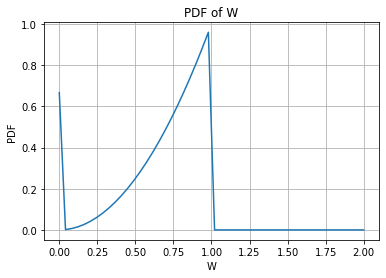
\includegraphics[width=\columnwidth]{assignment8pdf.png}
\end{center}
\end{figure}

\begin{figure}[htb!]
\begin{center}
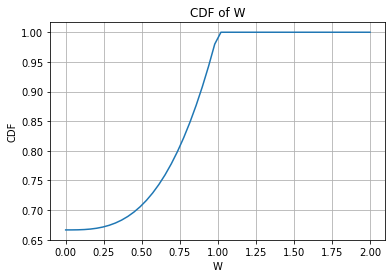
\includegraphics[width=\columnwidth]{assignment8cdf.png}
\end{center}
\end{figure}
\end{enumerate}
\end{document}